\documentclass[11pt]{article}

\usepackage{amssymb}
\usepackage{setspace}
\usepackage{amsmath}
\usepackage[T1]{fontenc}
\usepackage[utf8]{inputenc}
\usepackage{graphicx}
\usepackage[swedish]{babel}
\usepackage{fixltx2e}
\usepackage{subcaption}
\usepackage{placeins}
\usepackage{fancyhdr}
\usepackage{wrapfig}
\usepackage{tikz}
\usepackage{listings}
\usepackage{hyperref}
\usepackage{gensymb}

\newcommand{\dbar}{d\hspace*{-0.08em}\bar{}\hspace*{0.1em}}

\setlength{\intextsep}{5pt}
\setlength{\textfloatsep}{5pt}

\pagestyle{fancy}
\fancyhf{}
\rhead{SI1121}
\chead{\textbf{Värmepumpen}}
\lhead{Termodynamik}


\begin{document}

% -------- Section Title --------
\begin{titlepage}
	\centering
	{\scshape\LARGE Värmepumpen \par}
	{\scshape En introduktion för laborationsassistenter \par}
	\vspace{4cm}
	{\scshape\Large Termodynamik \\ SI1121\par}
	\vspace{2cm}
	\vfill
% Bottom of the page
	{\large \today\par}
\end{titlepage}

% -------- Section Förberedelsefrågor --------
\section{Förberedelsefrågor}

\subsection{Definiera termodynamikens andra lag}

\begin{equation}
    \mathrm{d}S \geq \frac{\dbar Q}{T}
\end{equation}

Detta förklarar varför vissa saker bara sker i en tidsriktning (kaffet kallnar i en kallare omgivning, universums värmedöd).

\subsection{Vilken relation mellan volym, tryck och temperatur är applicerbar i ett system med både gas och vätska?}

Van der Waals equation

\begin{equation}
    \left ( p + a \left ( \frac{n}{V} \right ) \right ) (V - nb) = nRT
\end{equation}


\subsection{Definiera entropi och entalpi}

\begin{equation}
    S = k_\text B \ln \Omega
\end{equation}
Entropi kan ses som ett mått på varje energikonfigurations sannolikhet, där $\Omega$ är antalet mikrotillstånd för ett givet makrotillstånd.

Visualisera ett system som kan anta ett set av mikrotillstånd, t.ex. luftpartiklar med hastigheter, som tillsammans ger ett makrotillstånd, t.ex. en temperatur. Vissa makrotillstånd kan fås genom fler mikrotillstånd än andra. Om alla mikrotillstånd har samma sannolikhet att förekomma, så kommer systemet gå till det makrotillstånd med flest antal mikrotillstånd.

Ett annat exempel som är något lättare att visualisera är hur många tillstånd ett ägg kan vara i efter det är krossat jämfört med innan.

\begin{equation}
    H = U + pV
\end{equation}
Entalpi kan enkelt beskrivas med hjälp av din egna kropp: Det är din inre energi, t.ex. värme eller de kemiskaprocesser som tillverkar värme i kroppen, plus den energi som det tar att trycka undan den volym luft som du upptar.  


% -------- Section Introduktion till pumpen --------
\section{Introduktion till pumpen}

\begin{itemize}
    \item Värmepumpen använder ett kylämne för att pumpa värme från en reservoar till en annan
    \item Kompressorn tillför arbete till systemet genom att komprimera och pumpa kylämnet
    \item Sex stycken temperaturmätare finns i systemet. Dessa manövreras med en ratt för att ändra vilken som syns på displayen
    \item Två stycken tryckklockor finns på varsin sida av systemet  
    \item En effektmätare mellan vägguttag och kompressorsladd (Denna måste stå på W och \underline{\textbf{inte}} MAX W)
\end{itemize}

% -------- Section Studentens arbetsuppgifter --------
\section{Studentens arbetsuppgifter}

\begin{itemize}
    \item Fyll upp de båda hinkarna med fyra liter vatten
    \item Gör en tabell och mät sex temperaturer, två tryck\footnote{Glöm ej att lägga på en bar då tryckklockorna mäter övertryck} och en effekt var femte minut i 40 minuter\footnote{Innan någon mätning kan göras så måste kompressorn stå på i 10 minuter}
    \item Med hjälp av mätvärdena, räkna ut `coefficients of performance' ($\epsilon_v, \ \epsilon$ och $\epsilon_C$)
    \item Rita processen i ett Mollierdiagram
\end{itemize}

% -------- Section Resultat och teori --------
\section{Resultat och teori}

\subsection{Coefficients of performance}

\begin{equation}
    \epsilon_v = \frac{Q_1}{W} = \frac{c_{\text{v}} m_{\text{v}} \Delta T}{\langle P \rangle t} \sim 1 \text{ till } 2
\end{equation}
Där $c_{\text{v}} = 4.2$ kJ/kg$\cdot$K vattens specifika värmekapacitet, $m_{\text{v}} = 4$ kg vattnets massa, $\Delta T$ är vattnets uppvärmda temperatur ($T_{\text{slut}} -T_{\text{start}}$), $\langle P \rangle$ medelvärdet av effekten, $t$ är den totala tiden.

\begin{equation}
    \epsilon = \frac{Q_2 + W}{W} = \frac{c_{\text{v}} m_{\text{v}} \Delta T + c_{\text{is}} m_{\text{is}} + \langle P \rangle t}{\langle P \rangle t} \sim 1 \text{ till } 2
\end{equation}
Där $c_{\text{is}} = 333$ kJ/kg är smältentalpin för vatten, och $m_{\text{is}} \approx 1$ kg isens massa\footnote{Om studenten vispar så halveras mängden is}. Observera att $\epsilon_v = \epsilon$ om inte systemet har några energiförluster.

\begin{equation}
    \epsilon_C = \frac{T_1}{T_1 - T_2} = \frac{\langle T_1 \rangle}{\langle T_1 \rangle - \langle T_2 \rangle} \sim 7 \text{ till } 9
\end{equation}
Där $T_i, \ i = 1, 2$ motsvarar temperatursensorn med samma nummer. $\epsilon_C$ beräknas för att göra en övre uppskattning på hur bra systemet kan vara. De två andra $\epsilon$ kan sedan jämföras med denna som

\begin{equation}
    \frac{\epsilon_v}{\epsilon_C} = \frac{\epsilon}{\epsilon_C} \sim 0.1 \text{ till } 0.3
\end{equation}

\subsection{Mollierdiagram}


\begin{figure}[h]
\centering
\begin{subfigure}{.5\textwidth}
  \centering
  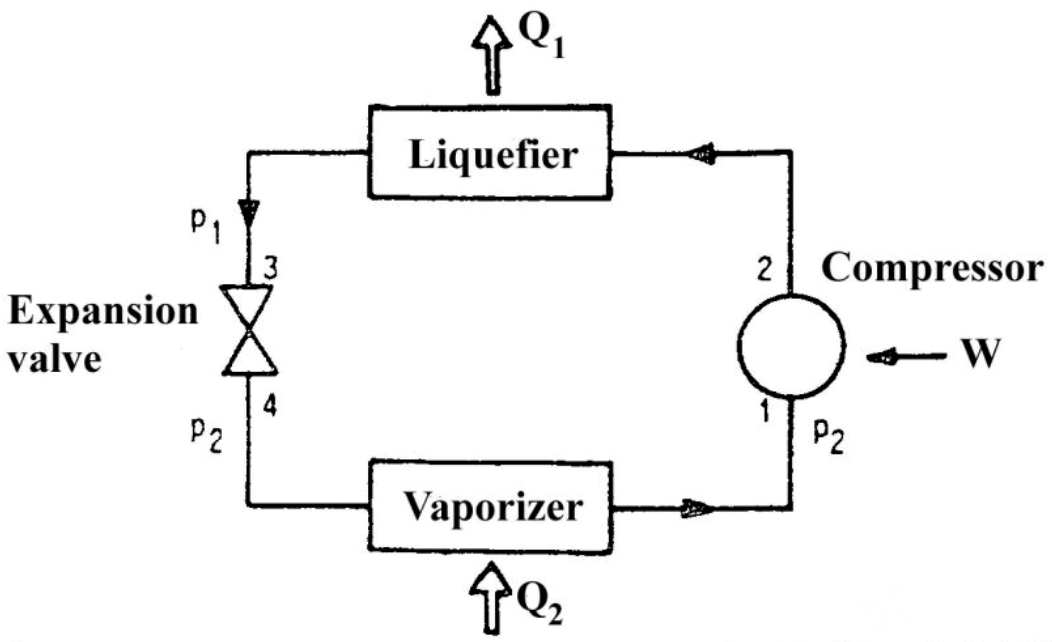
\includegraphics[width=1.08\linewidth]{BoxDiagram.png}
  \caption{Boxdiagram över värmepumpen}
  \label{Fig: Boxdiagram över värmepumpen}
\end{subfigure}%
\begin{subfigure}{.5\textwidth}
  \centering
  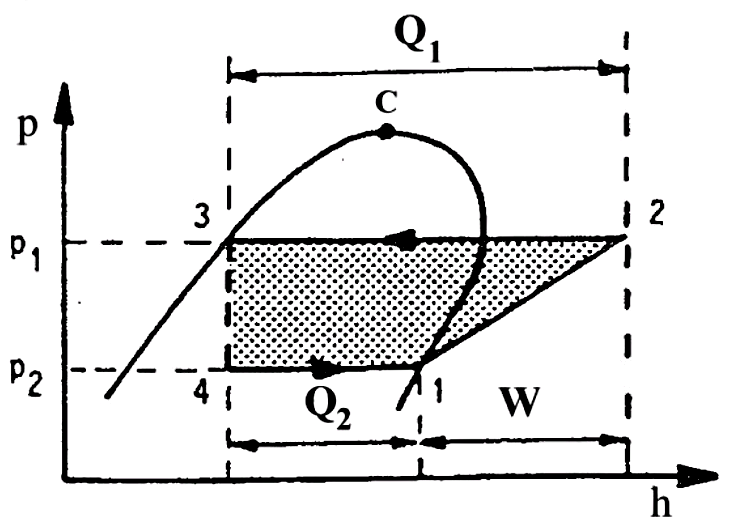
\includegraphics[width=.9\linewidth]{ProcessDiagram.png}
  \caption{Processen ritad i ett Mollierdiagram}
  \label{Fig: Processen ritad i ett Mollierdiagram}
\end{subfigure}
\caption{}
\end{figure}

Talen 1-4 i Figur \ref{Fig: Boxdiagram över värmepumpen} och \ref{Fig: Processen ritad i ett Mollierdiagram} motsvarar de hörn som grafen har. Genom att känna till vilka temperatursensorer, samt tryckklockor som motsvarar vilket hörn kan processen enkelt ritas ut.

\begin{table}[h]
\centering
\label{my-label}
\begin{tabular}{l|l|l}
Hörn & Temperatursensor & Tryckklocka      \\ \hline
1    & $T_5$            & $p_{\text{blå}}$ \\ \hline
2    & $T_6$            & $p_{\text{röd}}$ \\ \hline
3    & $T_2$            & $p_{\text{röd}}$ \\ \hline
4    & $T_1$            & $p_{\text{blå}}$ \\ \hline
\end{tabular}
\end{table}

Dessa ritas sen ut som $\langle T_i \rangle, \ \langle P_j \rangle$, då det endast är intressant hur processen rör sig ungefär varje varv.

% -------- Section Felkällor --------
\section{Felkällor}

\begin{itemize}
    \item Uppskattning av mängden is
    \item Osäkerheten i temperatursensorerna (de mäter bara hela \degree C)
\end{itemize}






\end{document}
